\documentclass[a4paper]{article}

\usepackage[french]{babel}
\usepackage[T1]{fontenc}
\usepackage[utf8]{inputenc}
\usepackage{amsmath}
\usepackage{graphicx}
\usepackage{lmodern}
\usepackage[left=3cm, right=3cm, bottom=4cm, top=4cm]{geometry}
\usepackage{array}
\usepackage{pdfpages}

\usepackage[gen]{eurosym}
\DeclareUnicodeCharacter{20AC}{\euro{}}

\usepackage{hyperref}
\hypersetup{    
    colorlinks,
    citecolor=black,
    filecolor=black,
    linkcolor=black,
    urlcolor=black
}

\title{Rapport de spécification}

\author
{
	Pierre-Marie {\sc Airiau}\\
    Valentin {\sc Esmieu}\\
    Hoel {\sc Kervadec}\\
    Maud {\sc Leray}\\
    Florent {\sc Mallard}\\
    Corentin {\sc Nicole}
}

\date{\today}

\newcommand{\pagevierge}[0]{\newpage\thispagestyle{empty}\null\newpage}

% Rapport de spécification fonctionnelle
%     Français
%     Décrire en détail les spécifications fonctionnelles du prj
%     Première idée architecture logicielle générale
%     décrire les grands modules et leur intéraction
%     Repart travail existant: Doit faire état tests effectués
%     Environ 20 pages


\begin{document}
    % Ouh c'est sale.
    \hypersetup{pageanchor=false}
    
\includepdf[pages=1]{figure/couv.pdf}
    \hypersetup{pageanchor=true}
    
    \newpage
    \thispagestyle{empty}
    \mbox{}
    
    \newpage
    % A decommenter pour la release
    % \setcounter{tocdepth}{2}
    \tableofcontents
    \setlength{\parskip}{10pt}
    
    \newpage
    \thispagestyle{empty}
    \mbox{}

    \newpage
    \section{Introduction}
	La sécurisation des systèmes est une problématique majeure de la société moderne. En ce sens, de nombreuses méthodologies ont été développées~\cite{introSecurite,ADTreeKordy} dans le but d'identifier les risques et de les quantifier. C'est avec cet objectif que le concept d'arbres d'attaque et de défense (ADTrees) a vu le jour.

	Lors de la phase de pré-étude, nous avons pu comprendre l’intérêt pratique de la construction des ADTrees. Leur utilisation permet d'identifier de manière précise les différentes attaques possibles contre un système et de les valuer en termes de coût, de probabilité, etc. ADTool~\cite{adtool_paper} (Attack-Defense Tree Tool), un logiciel libre développé pour l'implémentation de ces arbres sur support informatique, a été mis à disposition pour ce projet. Lors de sa prise en main, des limites ont été constatées. En effet, dans un cas concret d'expertise en sécurité, le système doit faire face à une multitude d'attaques possibles et, par conséquent, l'ADTree qui les modélisera sera de très grande taille. Dans ce cas, il est très difficile pour l'expert d'en extraire des informations pertinentes au premier coup d’œil. Or, ADTool ne fournit pas d'outil permettant à l'utilisateur de simplifier l'analyse de l'arbre. 

	L'objectif de ce projet est donc la création d'un logiciel intégrant ADTool et permettant de faciliter le travail d'un expert en sécurité, en lui fournissant des outils pour analyser facilement ses ADTrees. Ce logiciel portera le nom de \glasir{}  (prononcé [\textipa{glaziK}]). Il s'agit du nom d'un arbre aux feuilles d'or dans la mythologie nordique~\cite{vikingCulture}.

	Ce rapport présente les spécifications fonctionnelles de \glasir{}. Tout d'abord, les limites d'ADTool seront abordées, afin de justifier l'intérêt de \glasir{}. Puis nous détaillerons les différentes fonctionnalités destinées à l'analyse des ADTrees. Enfin, quelques améliorations supplémentaires seront également précisées pour offrir un meilleur confort de création et édition d'arbres. Ces spécifications seront faites en prenant en exemple une situation précise : celle d'un expert en sécurité chargé par le Service des Transports en commun de l'Agglomération Rennaise (STAR) de déterminer les failles de leurs systèmes de paiement.

    \section{Application}
	Notre logiciel sert à analyser la sécurité d'un système à l'aide d'ADTrees, de leur construction et de leur visualisation.

	Lorem ipsum dolor sit amet, consectetur adipiscing elit. Integer tempus luctus ex, non fringilla nibh laoreet non. Nullam sed enim nec leo dapibus tincidunt. Nulla augue est, cursus tempus tristique eget, venenatis sed leo. Nam eget purus lacinia, porttitor dolor eu, consectetur turpis. Suspendisse sed viverra tellus. Aliquam malesuada sed magna mattis dapibus. Pellentesque eu molestie ligula. Pellentesque dictum ultricies sagittis. Ut semper, est vitae malesuada facilisis, magna velit laoreet lectus, semper suscipit sapien lacus sed nulla.

	Aliquam finibus est ac cursus cursus. Fusce in libero ut nisi laoreet sodales. Cras vestibulum nec nulla in consequat. In eget lacus ut ipsum placerat ultrices. Nam diam magna, fermentum aliquam libero at, ornare eleifend diam. Sed et mi eget arcu bibendum congue. Vivamus in enim mollis, blandit sem in, hendrerit tellus.


	\subsection{Interface}
		Regardez comment la figure \ref{fig:interface} est jolie.

		\begin{figure}
			\begin{center}
				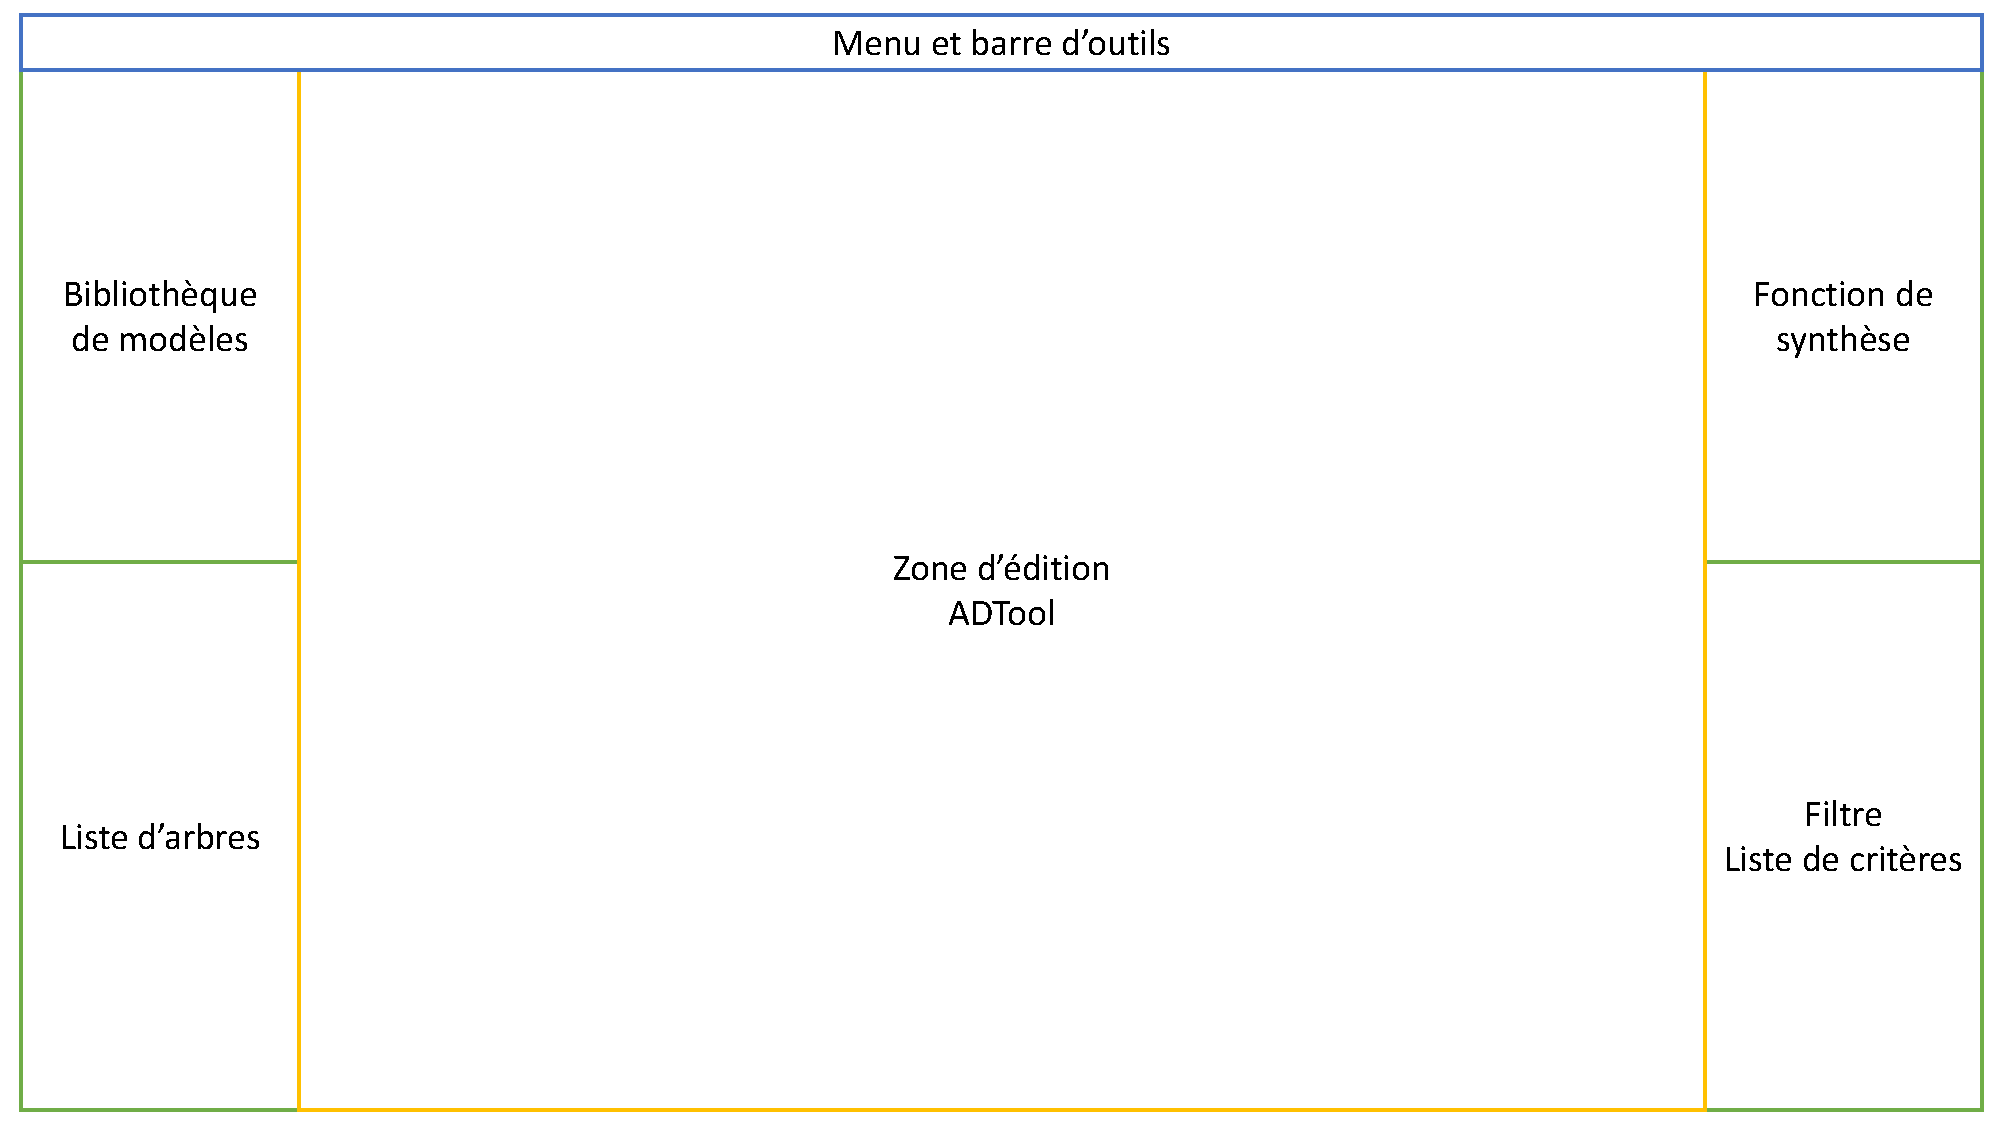
\includegraphics[width=1\textwidth]{figure/interface.pdf}
			\end{center}
			\caption{Là actuellement c'est la même figure que dans le rapport 1, on va changer ça.}
			\label{fig:interface}
		\end{figure}

		Maintenant on va expliquer l'interface et le fonctionnement général.

		Ensuite, on va détailler chaque module dans sa propre sous section. Chaque sous section contiendra une interface plus détaillée du module.

		Lorem ipsum dolor sit amet, consectetur adipiscing elit. Integer tempus luctus ex, non fringilla nibh laoreet non. Nullam sed enim nec leo dapibus tincidunt. Nulla augue est, cursus tempus tristique eget, venenatis sed leo. Nam eget purus lacinia, porttitor dolor eu, consectetur turpis. Suspendisse sed viverra tellus. Aliquam malesuada sed magna mattis dapibus. Pellentesque eu molestie ligula. Pellentesque dictum ultricies sagittis. Ut semper, est vitae malesuada facilisis, magna velit laoreet lectus, semper suscipit sapien lacus sed nulla.

		Aliquam finibus est ac cursus cursus. Fusce in libero ut nisi laoreet sodales. Cras vestibulum nec nulla in consequat. In eget lacus ut ipsum placerat ultrices. Nam diam magna, fermentum aliquam libero at, ornare eleifend diam. Sed et mi eget arcu bibendum congue. Vivamus in enim mollis, blandit sem in, hendrerit tellus.


	\subsection{Fichier projet}
	%	\begin{figure}
	%		\begin{center}
	%			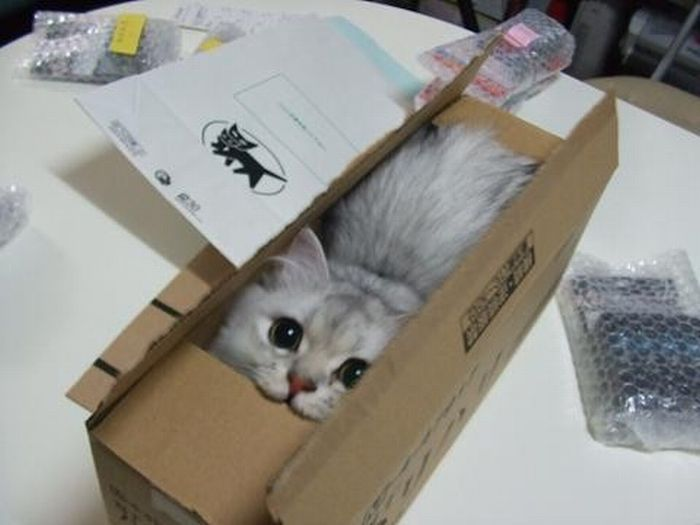
\includegraphics[width=1\textwidth]{figure/fichier.jpg}
	%		\end{center}
	%		\caption{Fichier}
	%		\label{fig:fichier}
	%	\end{figure}

		Mauris rhoncus tempor rhoncus. Vestibulum lacinia tincidunt sem ac auctor. Maecenas a lectus in nisi aliquet feugiat. Sed gravida laoreet maximus. Donec feugiat vestibulum neque sit amet mollis. Maecenas commodo luctus augue et molestie. Maecenas viverra semper massa, blandit commodo lacus blandit a. Proin sed euismod massa. Aenean nec nisl sed nisi mollis congue quis a nisi. Pellentesque habitant morbi tristique senectus et netus et malesuada fames ac turpis egestas. Suspendisse tincidunt euismod ipsum vitae commodo. Ut dapibus tellus nec libero egestas, eu venenatis dolor fermentum. Donec porttitor erat ante, at tincidunt lacus efficitur vitae.

		Vivamus elit urna, suscipit et nisi in, semper fringilla elit. In euismod cursus nunc quis tincidunt. Phasellus efficitur eleifend lacus, et pellentesque risus rhoncus vel. Phasellus in euismod lorem. Nam pulvinar aliquam metus a scelerisque. Etiam eget lectus ut felis porta ullamcorper. Aenean commodo at augue id pulvinar. Nunc efficitur elit est, id placerat sapien sodales nec. Etiam finibus at lacus nec viverra. Integer at vulputate mauris. Maecenas eget magna id tellus imperdiet finibus et in purus. Integer placerat ipsum a dui pellentesque, in lobortis lorem lobortis. In hac habitasse platea dictumst. 

	\subsection{Filtre}
		\begin{figure}
			\begin{center}
				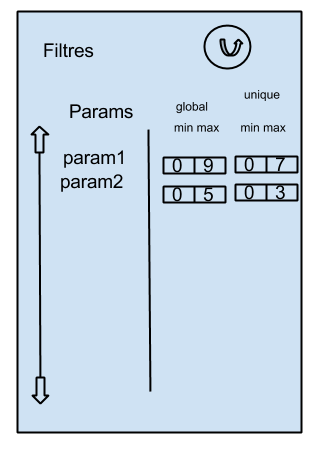
\includegraphics[width=0.25\textwidth]{figure/filtre.png}
			\end{center}
			\caption{Filtre}
			\label{fig:filtre}
		\end{figure}

		A l'heure actuelle, l'analyse d'arbre de grandes tailles à l'aide d'ADTool est difficile. En effet, ADTool a été pensé prioritairement pour la modélisation des systèmes sous forme d'ADTrees, et moins pour leurs analyses. ADTool met à disposition de l'expert, comme cela a été précisé précédemment, un certain nombre d'outils pour l'assister dans la modélisation de son système, parmi lesquels se trouve la valuation des noeuds de l'arbre. Une limite que présente ADTool est que, une fois le système à protéger complétement représenté sous la forme d'un ADTree, l'arbre peut être trop grand pour que l'expert puisse en retirer une information pertinante car le temps de parcours est trop long. 

		Le premier besoin qu'aura l'expert lors de l'analyse sera de rendre son arbre plus lisible, donc de le réduire. L'une des 

		En conséquence, l'analyse d'arbres à l'aide d'ADTool se fait principalement à la main, et devient donc impossible lorsque les arbres augmentent de tailles, faute à un support logiciel dédié.

		

		%\begin{itemize}
		  %\item bouton pour ajouter nouveau paramètre sur le filtre (par default : pas de filtre => pas de paramètres) 
			 % \begin{itemize}
			  	% \item ajouter ouvre selection de paramétres : menu déroulant précisant les paramètres disponibles.
			  %\end{itemize}
		  %\item tous les paramètres ont à coté d’eux deux sections : une de filtre global et une de filtre unitaire. Dans le filtre global sont présentes deux %cases, une nommée “min” et une nommée “max”. De même dans le filtre unitaire.
		 % \item par défaut, les min sont moins l'infini et les max sont l’infini (pas de filtre)
		  %\item il est possible d’inscrire des valeurs dans les cases “min” et “max” afin de réduire l’intervalle de sélection des branches de l'arbre.
		  %\begin{itemize}
			  	 %\item la section globale permet de conserver les branches de l’arbre dont la valeur totale du paramètre se trouve dans l’intervalle. (ex %: entre 500 et 1000 euros au total)
			  	% \item la section unitaire permet de conserver les branches de l’arbre dont chacune des valeurs de chacune des feuilles se trouve dans %l’intervalle. (ex : pas de dépenses de moins de 10 euros et pas de plus de 100 euros)
		 % \end{itemize}
		  %\item il est ainsi possible de combiner les critères de sélection (ex : entre 500 et 1000 euros au total et pas de dépenses de moins de 10 euros %et pas de plus de 100 euros ; et le temps entre X et Y et ….)
		 % \item barre de défilement pour les cas de surcharge de paramètres
		  %\item possibilité d'activer ou désactiver les paramètres ( bouton a cocher)
		  %\item bouton ``générer'' permet de créer un nouvelle arbre filtré en fonction des paramètres définie. Il est ouvert dans un nouvelle onglet de la %section ADTool de l'interface. 
		 % \item chaque arbre posséde son propre outil filtre. Lors de la génération, le nouvelle arbre posséde un outil filtre vide. 
		  %\item le nouvel arbre posséde un commentaire : filtre depuis l'arbre X avec paramétre Y, heure, version. \ldots
		  %\end{itemize}


	\subsection{Editeur de fonction}
		\begin{figure}
			\begin{center}
				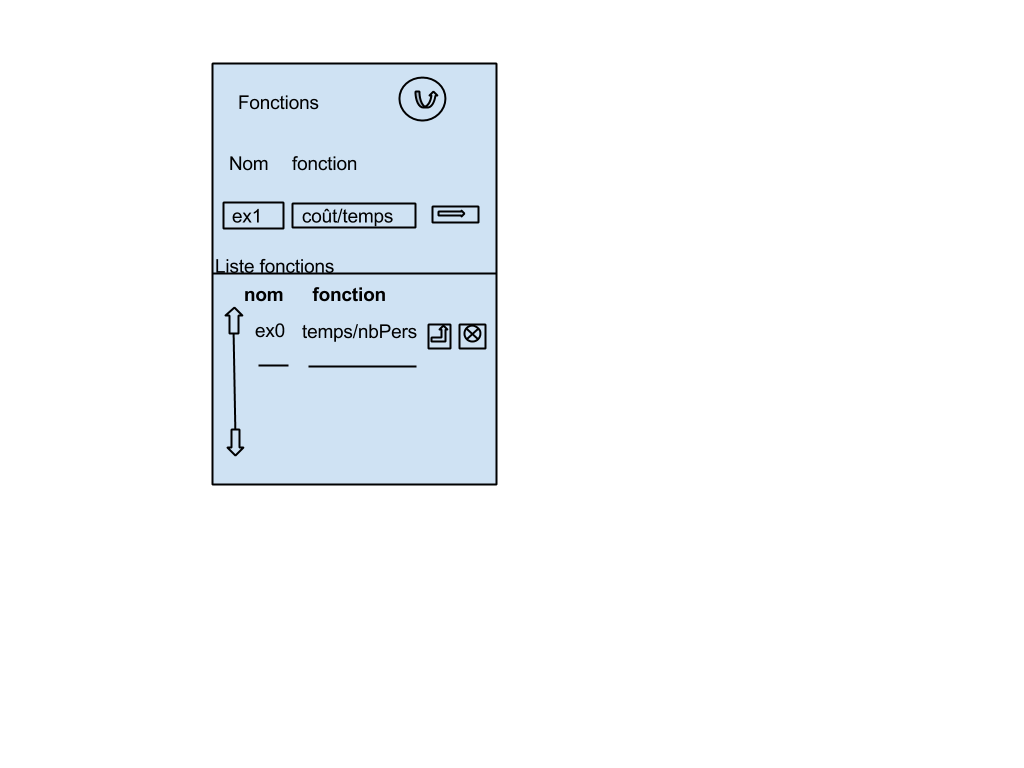
\includegraphics[width=0.25\textwidth]{figure/fonction.png}
			\end{center}
			\caption{Fonction}
			\label{fig:fonction}
		\end{figure}

		\begin{itemize}
			\item (présence préallable de 6 valuations de synthèse définies dans ADTool, et non instanciées par défaut. )
			\item décomposition en deux zones : une pour l'édition du nouveau paramètre et de sa fonction, et une pour le rappel des fonctions déjà existantes.
			\item Zone 1 : Présence d’un menu déroulant pour choisir laquelle des 6 valuation de synthèse est à instancier, et d'une zone textuelle pour écrire la fonction qu'on lui associe. La fonction est une fonction linéaire ou non, et qui prend en paramètres des valuations de l'arbre déjà définies (dans ADTool ou d'autres fonctions de synthèse). Bouton à coté pour valider la création. Si echec de la création (fonction non valable, etc.), message d'erreur donné par le guide (avec conseils éventuels).
			\item zone 2 : présence en dessous de la zone 1 d’une zone de rappel des fonctions de synthèse déjà instanciées. A coté de chacune d’entre elles il y a deux boutons : un pour modifier une fonction déjà créée, et un autre pour la supprimer.
			\item bouton “actualiser” en haut pour mettre à jour la liste des fonctions. \ldots
		\end{itemize}
		
		
		


	\subsection{Bibliothèque de modèles}
	%	\begin{figure}
	%		\begin{center}
	%			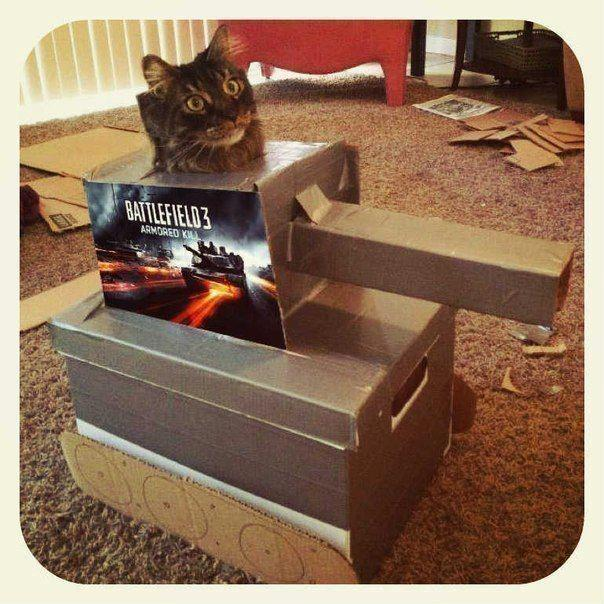
\includegraphics[width=1\textwidth]{figure/biblio.jpg}
	%		\end{center}
	%		\caption{Biblio}
	%		\label{fig:biblio}
	%	\end{figure}

		\begin{itemize}
			\item Le logiciel posséde une bibliothéque par défault
			\item la création d'un projet crée une nouvelle bibliothéque, copie de la bibliothéque par défault
			\item la bibliothéque est contenue dans le fichier projet de l'utilisateur. 
			\item Permet un accès facile à tous les arbres stockés
			\item bouton “actualiser” en haut pour mettre à jour la liste des fonctions.
			\item Regroupe les arbres par catégorie (par catégorie d’attaquant, de type d’attaque…), vue en arborescense. 	donner des types aux arbres stockés ?
			\item Permet d’y ajouter des éléments (géré automatiquement lors de la création dans un projet ?) Si non, bouton “ajouter” pour l’arbre courant. 
			\item Retirer des éléments : permet de retirer un élément et mettre à jour la bibliothèque, utile en cas d’arbre faux, ou considéré comme pas assez général pour servir de modèle. (cohérence avec l’ajout d’arbres)
			\item Pouvoir rechercher un arbre dans les modèles généraux (aussi rôle du guide) mais guide facultatif. Série de questions pour pouvoir sélectionner des modèles.
			\item Possibilité d'ajouter des arbres dans la bibliothéque par défault.\ldots
		\end{itemize}
		


	\subsection{Liste d'arbres}
	%	\begin{figure}
	%		\begin{center}
	%			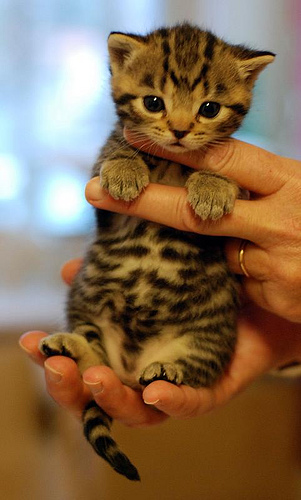
\includegraphics[width=0.5\textwidth]{figure/liste.png}
	%		\end{center}
	%		\caption{Liste}
	%		\label{fig:liste}
	%	\end{figure}


		\begin{itemize}
			\item Liste d'arbres générés par l'utilisateur puis sauvegardés sous différentes catégories/sous-catégories (arborescence)
			\item Au départ, une seule catégorie défaut
			\item  Création des catégories + possibilité d'affiner en sous-catégories
			\item Suppression d'une catégorie supprime tous les arbres compris dedans
			\item bouton “actualiser” en haut pour mettre à jour la liste des fonctions.
			\item Glisser/déposer les arbres pour les déplacer entre les catégories
			\item Possibilité de supprimer les arbres (renommer aussi ?)
			\item Double-clic pour ouvrir les arbres dans une fenêtre ADTool.\ldots
		\end{itemize}
		

	\subsection{Guide}
	%	\begin{figure}
	%		\begin{center}
	%			
\includegraphics[width=1\textwidth]{figure/guide.jpg}
	%		\end{center}
	%		\caption{Guide}
	%		\label{fig:guide}
	%	\end{figure}

		\begin{itemize}
			\item À activer dès la création du projet, possibilité de supprimer à tout moment 
			\item SAD peut aussi donner quelques conseils au début, genre raccourcis clavier), avec possibilité de désactiver
			\item Il peut aussi présenter le menu d'accueil du logiciel (Créer nouveau projet, etc)
			\item Donne des indications (genre Ouvre un nouveau projet) avec un bouton Suivant			
			\item SAD indique les erreurs (comme celles dans l'éditeur de fonctions), en gros toutes les exceptions levées par le logiciel\ldots
		\end{itemize}


	\subsection{Éditeur d'arbres}

		Attention: on ne parlera ici que de l'intéraction entre l'éditeur et les différents modules, pas de l'éditeur en lui même.
		Voir la section \ref{sec:adtool} pour voir nos améliorations.

		\begin{itemize}
			\item  Utilisation d'ADTool imbriqué dans l'IHM
			\item Une instance d'ADTool par arbre (possibilité d'ouvrir plusieurs onglets) : modèles, filtres, etc
			\item Chaque modification dans ADTool entraine une mise à jour de SAD
			\item Sauvegarde des fichiers par ADTool : ne pas laisser le choix du fichier, laisser seulement le fichier projet (en gros, l'arborescence d'arbres)\ldots
		\end{itemize}


    \section{ADTool}
	\label{sec:adtool}

	Présentation des tests et des limitations actuelles.

	\subsection{Couper copier coller}
	
	- Sélection d'un noeud (ça sélectionne aussi ses fils) : repérée par une coloration du noeud sélectionné
	- Clic droit sur le noeud sélectionné pour le copier/couper ainsi que ses fils
	- Pour coller on clique droit sur un noeud et cela rajoute l'arbre copié en tant que nouveau fils
	- On peut le faire entre différentes instances d'ADTool
	- Sanity check : faire attention au nom des labels

	\subsection{Amélioration XML}

	- Ajouter la possibilité d'éditer l'arbre directement en xml. Possibilité de masquer/afficher le bloc xml.
	- Ajouter noeud père dans l'éditeur texte 
	
	\subsection{CTRL-Z}

	- Annulation d'une ou plusieurs des modifications précédentes
	- Coder une pile d'états avec un curseur qui indique l'état courant
	- Chaque action entraîne la création d'un nouvel état
	
	\subsection{Paramètre de synthèse}
	- ajouter un paramètre de plus de disponible dans AdTool pour les fonctions de synthése.
		
	\subsection{Vue globale des paramètres}

	- Pour le moment, un onglet dans ADTool par paramètre (sur l'arbre, seul ce paramètre est apparent)	
	- Créer un nouvel onglet plus global avec tous les paramètres visibles sous les labels, chaque paramètre d'une couleur différente (légende explicative sur le coté)
	- Attention à ce que les paramètres ne débordent pas des noeuds, il faut éventuellement élargir les ronds

    \section{Organisation}
	\label{sec:orga}
	\subsection{La méthode SCRUM}
		\label{subsec:scrum}

	Afin de définir la méthode de gestion de projet à mettre en place pour la réalisation de \glasir{}, nous avons débattu ensemble des différentes méthodes à notre disposition. A la suite de 	nos discussions en réunions, nous nous sommes dirigés vers une méthode agile proche du \og \textsc{scrum} \fg{}. Ce choix s'est fait sur les points qui sont détaillé ci-dessous :

	L'organisation des rôles que nous avons mise en place depuis le début du projet se base sur un rôle de \og Coordinateur \fg{}, qui est responsable de la réalisation et du rendu d'un livrable (rapport, version logicielle, etc). Ce rôle tourne à chaque nouveau livrable, de sorte que chacun des membres de l'équipe l'exerce au moins une fois. Le rôle de coordinateur que nous avons défini nous a donc semblé correspondre au rôle de ScrumMaster tel que défini dans la méthode \textsc{scrum}.

	Le coordinateur endosse également la responsabilité de Product Owner, qu'il partage avec les encadrants du Projet pour ce qui est de la définition des Objectifs et surtout de l'acceptation des livrables.

	En place de la mêlée quotidienne du \textsc{scrum}, nous nous réunissons une fois par semaine afin de discuter de l'avancement de nos tâches respectives et faire part de nos difficultés. Nous avons décidé d'adopter un rythme hebdomadaire plutôt que quotidien car nous ne travaillerons pas à temps plein sur le projet et ce rythme nous a donc semblé plus adéquat. Nous définissons en fonction des retours en réunion les éventuels ajustements à effectuer la semaine suivante et dans le reste de la planification.

	Enfin, chaque version sera composée de sprints au cours desquels nous nous consacrerons à un sous-ensemble de tâches nécessaires à la réalisation d'une version de \glasir{}. Ces tâches constitueront les Users Stories du projet, et sont détaillées dans la \textsc{sous-section}~\ref{subsec:taches_unitaires}.  
	
	\subsection{Tâches unitaires et estimations}
		\label{subsec:taches_unitaires}

	Nous avons décidé de livrer trois versions de \glasir{} : deux intermédiaires et une finale. Ces dernières ont elles-mêmes été divisées en tâches unitaires, décrites dans cette section.
	
	Pour déterminer le temps nécessaire à l'accomplissement de chaque tâche, nous avons combiné les méthodes d’estimation \og Analogique \fg{} et \og Expertise \fg{}. En effet, la méthode \og Analogique \fg{} consiste à estimer la durée d'une tâche par analogie avec une tâche similaire déjà effectuée (au sein d'un autre projet par exemple). La méthode \og Expertise \fg{}, quant à elle, repose sur le jugement d'un expert. Bien qu'aucun membre de notre groupe ne puisse réellement se considérer comme tel, nos stages respectifs ont tout de même permis d'apporter des avis constructifs sur l'estimation de la durée des tâches.
	
	Les résultats de ces différentes estimations sont décrits ci-après pour chaque version. Il est à noter que les tests et la rédaction de la documentation sont pris en compte dans l'estimation du temps nécessaire à la réalisation de chacune des tâches.
	

		\subsubsection{Version 0.1}
			Huit grandes tâches ont été identifiées pour cette version et sont présentées dans la {\sc Table} \ref{tab:taches_units_1}. 
			\begin{table}[H]
				\centering
				\begin{tabular}{|c|r|l|c|r|}
					\hline
					\textbf{Cible} & \textbf{Id} & \textbf{Tâche} & \textbf{Technologies} & \textbf{Durée}\\
					\hline

					\multirow{5}{*}{\glasir{}} & 1.1 & Squelette interface & WPF & 6h\\
					\cline{2-5}
					 & 1.2 & Gestion fichiers projet & C++ & 20h\\
					\cline{2-5}
					 & 1.3 & Intégration ADTool dans \glasir & JNI & 20h\\
					\cline{2-5}
					 & 1.4 & \'Evaluateur de fonction & Java & 12h\\
					\cline{2-5}
					 & 1.5 & Interface évaluateur & WPF & 8h\\
					\hline

					\multirow{3}{*}{ADTool} & 1.6 & Valuation ADTrees & \multirow{3}{*}{Java} & 18h\\
					\cline{2-3} \cline{5-5}
					 & 1.7 & Refonte langage des ADTrees & & 16h\\
					\cline{2-3} \cline{5-5}
					 & 1.8 & Vue globale des paramètres & & 12h\\
					\hline

					\multicolumn{4}{|l|}{\bf Total} & {\bf 112h}\\
					\hline
				\end{tabular}
				\caption{Tâches associées à la version 0.1.}
				\label{tab:taches_units_1}
			\end{table}
			
			
			La réalisation de cette version sera découpée en trois sprints, présentés ci-dessous :

			\noindent\textbf{Sprint 1} Création de l'interface utilisateur de base de \glasir{}, intégration du logiciel ADTool en tant que fenêtre de \glasir{}, possibilité de création d'un nouveau projet et sa sauvegarde, affichage des différents arbres d'un projet dans un dock sous forme d'arborescence.\newline
			\textbf{Sprint 2} Reconnaissance d'une formule mathématique par le logiciel ADTool, création d'un paramètre en fonction de l'évaluation de cette formule, et l'amélioration de la représentation des arbres sous forme d'une grammaire au sein d'ADTool.\newline
			\textbf{Sprint 3} Affichage de plusieurs paramètres par nœud d'un arbre, possibilité de communication entre le module éditeur de fonction de \glasir{} et la partie création d'un paramètre de synthèse implémentée précédemment dans ADTool.\newline


		\subsubsection{Version 0.2}
			Le développement de la version 0.2 est découpé en cinq tâches, visibles dans la {\sc table} \ref{tab:taches_units_2}.
			\begin{table}[h]
				\centering
				\begin{tabular}{|c|r|l|c|r|}
					\hline
					\textbf{Cible} & \textbf{Id} & \textbf{Tâche} & \textbf{Technologies} & \textbf{Durée}\\
					\hline

					\multirow{4}{*}{\glasir{}} & 2.1 & Algorithme filtrage & C++ & 24h\\
					\cline{2-5}
					 & 2.2 & Interface filtre & WPF & 15h\\
					\cline{2-5}
					 & 2.3 & Multiples instances d'ADTool & C++, WPF & 20h\\
					\cline{2-5}
					 & 2.4 & Affichage arbre filtré & Java, WPF & 16h\\
					\hline

					\multirow{1}{*}{ADTool} & 2.5 & Couper/copier/coller & \multirow{1}{*}{Java} & 25h\\
					\hline

					\multicolumn{4}{|l|}{\bf Total} & {\bf 100h}\\
					\hline
				\end{tabular}
				\caption{Tâches associées à la version 0.2.}
				\label{tab:taches_units_2}
			\end{table}
			
			Nous avons réparti les tâches en trois sprints :

			\noindent\textbf{Sprint 4} Implémentation de l'algorithme de filtrage, permettre l'ouverture de plusieurs instances d'ADTool au sein de différents onglets de l'interface de \glasir{}.\newline 
			\textbf{Sprint 5} Affichage du panneau relatif à ce module au sein de l'interface utilisateur de \glasir{}. Implémentation de la fonction couper/copier-coller.\newline % ou durant le snd sprint?
			\textbf{Sprint 6} Affichage de l'arbre filtré.

		\subsubsection{Version 1.0}
			Quatre tâches ont été identifiées pour la version 1.0 de \glasir{}, regroupées dans la {\sc Table} \ref{tab:taches_units_3}.
			\begin{table}[h]
				\centering
				\begin{tabular}{|c|r|l|c|r|}
					\hline
					\textbf{Cible} & \textbf{Id} & \textbf{Tâche} & \textbf{Technologies} & \textbf{Durée}\\
					\hline

					\multirow{4}{*}{\glasir{}} & 3.1 & Optimiseur & C++, WPF & 30h\\
					\cline{2-5}
					 & 3.2 & Bibliothèque de modèles & C++, WPF & 20h\\
					\cline{2-5}
					 & 3.3 & Harmonisation interface & WPF & 16h\\
					\cline{2-5}
					 & 3.4 & Packaging & ? & 8h\\
					\hline

					\multirow{1}{*}{ADTool} & 3.5 & Ctrl-Z & \multirow{1}{*}{Java} & 16h\\
					\hline

					\multicolumn{4}{|l|}{\bf Total} & {\bf 90h}\\
					\hline
				\end{tabular}
				\caption{Tâches associées à la version 1.0.}
				\label{tab:taches_units_3}
			\end{table}
			
			Les sprints se composeront de :

			\noindent\textbf{Sprint 7} Implémentation de l'algorithme de l'optimiseur, création d'une bibliothèque de modèles.\newline
			\textbf{Sprint 8} Affichage du panneau de l'optimiseur dans \glasir{}, possibilité d'annuler une action dans ADTool.\newline
			\textbf{Sprint 9} Harmonisation de l'interface et réalisation du packaging. \newline

		%TODO estimations
	\subsection{Organisation du groupe et répartition des tâches}
		Lors de la phase de développement de \glasir{}, notre groupe de projet sera réduit à trois étudiants : Pierre-Marie {\sc Airiau}, Valentin {\sc Esmieu} et Maud {\sc Leray}. Les trois autres, Florent {\sc Mallard}, Hoel {\sc Kervadec} ainsi que Corentin {\sc Nicole}, partiront en effet étudier à l'étranger.
		
		Nous comptons donc nous répartir les tâches selon trois composantes générales : Maud L. travaillera principalement sur ADTool, Pierre-Marie A. sur les algorithmes et sur l'interfaçage entre ADTool et \glasir{}, et Valentin E. s'orientera sur l'interface utilisateur de \glasir{}. La {\sc Table} \ref{table:repartition} donne la répartition des tâches plus en détails.
			


		\begin{table}[H]
			\centering
			\begin{tabular}{|l|c|r||c|r||c|r|}
				\hline
				\multirow{2}{*}{} & \nomRepart{Pierre-Marie A.} & \nomRepart{Valentin E.} & \nomRepartt{Maud L.}\\
				\cline{2-7}
				 & {\bf Id tâche} & {\bf Durée} & {\bf Id tâche} & {\bf Durée} & {\bf Id tâche} & {\bf Durée}\\
				\hline
				{\bf Version 0.1} & - & {\bf 38h} & - & {\bf 34h} & - & {\bf 40h}\\
				 & 1.3 & 10h & 1.1 & 6h & 1.2 & 10h\\
				 & 1.4 & 12h & 1.2 & 10h & 1.6 & 18h\\
				 & 1.7 & 16h & 1.3 & 10h & 1.8 & 12h\\
				 & - & - & 1.5 & 8h & - & -\\
				\hline
				{\bf Version 0.2} & - & {\bf 39h} & - & {\bf 33h} & - & {\bf 28h}\\
				 & 2.1 & 24h & 2.3 & 20h & 2.4 & 16h\\
				 & 2.2 & 15h & 2.5 & 13h & 2.5 & 12h\\
				\hline
				{\bf Version 1.0} & - & {\bf 25h} & - & {\bf 23h} & - & {\bf 42h}\\
				 & 3.1 & 15h & 3.1 & 15h & 3.2 & 10h\\
				 & 3.2 & 10h & 3.4 & 8h & 3.3 & 16h\\
				 & - & - & - & - & 3.5 & 16h\\
				\hline
				{\bf Total} & \multicolumn{2}{r||}{{\bf 102h}} & \multicolumn{2}{r||}{{\bf 100h}} & \multicolumn{2}{r|}{{\bf 110h}}\\
				\hline
			\end{tabular}
			\caption{Répartition des tâches, par personne et par version.}
			\label{table:repartition}
			\label{tab:repartition}
		\end{table}


	\subsection{Risques}
		\label{subsec:risques}

	%L'implémentation d'un logiciel comporte toujours des risques. Afin de ne pas nous laisser surprendre par ces derniers, nous avons cherché à lister ceux qui nous venaient à l'esprit.

    % Pour que notre projet se déroule le mieux possible, nous avons listé certains événements susceptibles de nous faire prendre du retard. Ils sont répertoriés dans le tableau\ref{fig:risques}, avec les tâches qu'ils concernent. Nous leur avons ajouté les notions de probabilité (Pr) et de criticité (Cr), sur une échelle de 1 à 3 : 1 pour faible, 2 pour moyenne, 3 pour élevée. Enfin, la dernière colonne cite des solutions possibles pour contre les risques énoncés.

    Dans le but de délivrer ce projet dans les délais, une évaluation des risques a été effectuée. Celle-ci a pour but d'identifier les différents facteurs qui pourraient engendrer des difficultés dans la réalisation des tâches et entraîner ainsi un retard, ou une incapacité à implémenter une partie du cahier des charges. Nous avons associé à chaque élément de cette liste les notions de probabilité (Pr) et de criticité (Cr), sur une échelle de 1 à 3 : 1 pour faible, 2 pour moyenne, 3 pour élevée. Dans le but de réagir au mieux en cas d’apparition de ces aléas, des solutions ont été définies. Le résultat de cette réflexion est présenté dans la \textsc{table}~\ref{fig:risques}. 


	\begin{table}[H]
		\centering
		\begin{tabular}{|p{4cm}|l|l|l|p{4cm}|}
		\hline
            \textbf{Risque} & \textbf{Tâches concernées} & \textbf{Pr.} & \textbf{Cr.} & \textbf{Solution}\\
            \hline
            Mauvaise estimation des durées nécessaires aux tâches unitaires & 
                Toutes & 3 & 3 &
                Bien s'organiser et respecter les délais\\ 
            \hline
            Apparition d'un bug difficile à corriger & 
                Toutes & 3 & 3 &
                Faire des tests unitaires\\
            \hline
            Difficulté à créer une grammaire & 
                1.4 & 1 & 2 &
                Simplifier les expressions à évaluer\\ 
            \hline
            Manque de connaissances techniques & 
                Toutes & 3 & 3 &
                Approfondir nos connaissances\\ 
            \hline
            Rédaction trop tardive de la documentation & 
                Toutes & 2 & 1 &
                Commenter le code au fur et à mesure\\
            \hline
            Mauvaise compréhension du code d'ADTool & 
                Toutes celles sur ADTool & 2 & 2 &
                Contacter le développeur d'ADTool\\ 
            \hline
            Mauvaise communication entre ADTool et \glasir{} & 
                1.4, 2.1, 3.1 & 2 & 3 &
                Utiliser le fichier XML lisible par ADTool\\ 
            \hline
            Perte de temps sur une tâche secondaire & 
                Toutes & 2 & 1 &
                Compter ses heures, faire le point lors des réunions\\ 
            \hline
            Algorithme ralentissant le logiciel & 
                3.1, 2.2 & 1 & 1 &
                Optimiser l’algorithme\\ 
            \hline
            Échec de l'intégration d'ADTool dans \glasir{} & 
                1.2 & 1 & 3 &
                Lancer ADTool séparément\\ 
            \hline
		\end{tabular}
		\caption{Tableau des risques}
		\label{fig:risques}
	\end{table}
	

    \section{Critiques}
	Après la rédaction du rapport précédent (pré-étude), nous avions constaté que notre organisation de travail était à revoir. 
	En effet, nous avions trop cloisonné la rédaction des différentes parties, et il nous manquait un superviseur chargé d'harmoniser le tout.
	Le résultat fut un rapport dont les parties ne s'enchaînaient pas toujours correctement, et avec des styles de rédaction très variables : cela manquait d'homogénéité.

	De plus, nous avions trop tardé à faire nos \og brainstorming \fg~ pour déterminer précisément ce que nous allions faire, ce qui a grandement retardé la rédaction. Nous avons même dû supprimer une partie de notre travail.

	À partir de ces constats, nous avons décidé de démarrer ce deuxième rapport par une série de réunions. Cela nous a permis de commencer la rédaction en ayant une idée précise de ce que nous allions écrire.
	Cette fois, nous avons désigné un responsable d'harmonisation, Corentin Nicole, qui rédige moins mais s'assure de la cohérence globale du rapport tout au long de son avancement.

% ABSENCE DE REFERENCES

    % On a pas de conclusion :o

    % a eviter
    \nocite{*}

    \bibliographystyle{plain}
    \bibliography{input/biblio}

    % Manoucherie incoming
    \pagevierge
    \ifthenelse{\isodd{\thepage}}
    {\pagevierge}
    {}
    
\includepdf[pages=2]{figure/couv.pdf}
\end{document}